\chapter{Robot de pruebas}
\label{chap:robot}

Con la finalidad de demostrar y hacer un primer uso de la aplicación se ha decidido abordar la elaboración de un vehículo de pruebas. Dicho vrhículo será utilizado de modelo o gúia para el 
resto de personas que quieran crear un robot para su integración en la aplicación o bien para programar un robot del que y dispongan previamente.\\

En el presente capítulo se detalla los diferentes pasos que se han seguido a la hora de la construcción y programación del vehículo a modo de guía y ejemplo paso a paso \footnote{aclaracion: esto es una aclaración.}.\\


\begin{figure}[H]
  \begin{center}
    \includegraphics[scale=0.2]{imagenes/robot2.jpg}
  \end{center}
  \caption{Imagen del robot de pruebas.}
  \label{robot:robot02}
\end{figure}


\section{Análisis}
\ref{sec:analais}




\subsection{Análisis de requerimientos hardware}
\label{sec:requerimientos-hardware}

Se ha optado por la construcción de un  pequeño robot móvil dotado de un chasis de 4 ruedas donde cada una de ellas está accionada por un motor. Los motores seleccionados funcionan a corriente continua
de manera que en función de la polarización de los terminales hace girar las ruedas en una dirección o la contraria (marcha adelante o atrás).\\

El chasis seleccionado permite añadir multitud de componentes que desees para construir tu robot gracias a sus dos paneles para instalar las diferentes
placas electrónicas y sensores.\\

El robot además necesita de una cámara para la obtención de vídeo y su transmisión. Para ello se ha empleado una cámara de pequeñas dimensiones de alta definición.\\

Por otra parte, todo robot necesita de una unidad de central de procesamiento donde se localizará el programa de control. Este programa tendrá la función de interpretar las diferentes señales recibidas,
control de sensores y dispositivos conectados. Además, esta placa es la encargada de distribuir la alimentación por los diferentes componentes hardware que lo necesiten y recibir las señales de
los sensores y enviarla a los motores. Utilizando para ello la placa Raspberry Pi modelo B cuya descripción se encuentra en la sección \ref{}.\\

Este modelo de placa dispone de  una serie de pines denominados GPIO (General Purpose Input/Output) que son, como su propio nombre indica, un sistema de E/S (Entrada/Salida) de propósito general,
es decir, una serie de conexiones que se pueden usar como entradas o salidas para usos múltiples. Estos pines están incluidos en todos los modelos de Raspberry Pi, con la
finalidad de ser utilizados en diferentes proyectos de una manera similar a la que se haría con Arduino\footnote{Arduino es una plataforma de prototipos electrónica de código abierto (open-source) 
basada en hardware y software flexibles y fáciles de usar.}

\section{Análisis de requerimientos de Software}

Habiendo detallado los requerimientos hardware para la construcción del robot, pasamos al análisis del programa implementado para su correcto funcionamiento.\\

La programación del robot uno de los requisitos fundamentales era el de disponer de una vía de comunicación bidireccional.\\

Para ello se ha seleccionado el entorno de ejecución Node.Js, el cual permite escribir programas en JavaScript además de disponer de una gran cantidad de bibliotecas hechas por toda una comunidad que la respalda.
Además de que permite escribir programas relativamente complejos en tan sólo unas pocas líneas de código.\\

se ha realizado haciendo uso de Websockets los cuales presentan algunas ventajas sobre simples solicitudes http:

\begin{itemize}
 \item Velocidad: Una petición http normal tiene que establecer una conexión antes de comenzar las transacciones, la cual toma bastante tiempo. 
 Los Websockets, una vez establecida la conexión, siempre están abiertos y listos para enviar o recibir datos. Esto significa que el retraso puede ser tan bajo como su ping,
 en torno a un milisegundo o dos en la mayoría de los casos.
 \item Bidireccional: Los Websockets permiten transmisión de datos en ambas direcciones permitiendo la activación de eventos en el cliente y viceversa.
\end{itemize}

Como podemos ver las propiedades anteriormente descritas resultan esenciales para nuestro proyecto que, como cabe recordar, queremos realizar lectura de sensores y envío de órdenes desde un servidor externo. Además de 
la transmisión de vídeo.\\

\section{Montaje}

En esta sección se recogen todas las descripciones y procedimientos seguidos y que han resultado de mayor interés a la hora de la construcción del robot y sus diferentes interconexiones.\\

\subsection{Interconexión de elementos}

En la sección \ref{} se describen los diferentes elementos hardware que han sido necesarios para la construcción del vehículo.\\

Para la placa Raspberry Pi Model B+, los pines GPIO se encuentran distribuidos de la siguiente manera:

\begin{figure}[H]
  \begin{center}
    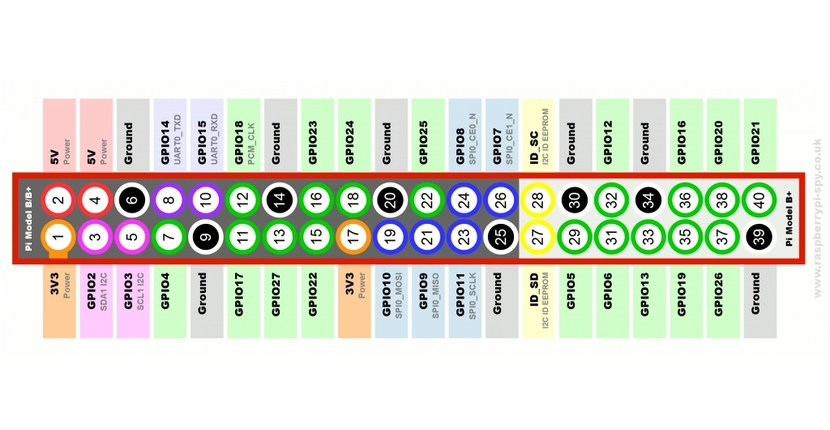
\includegraphics[scale=0.4]{imagenes/robot/gpio-conexiones.jpg}
  \end{center}
  \caption{Esquema GPIO de una Raspberry Pi Model B+.}
  \label{gantt:tareas01}
\end{figure}

Los pines empleados son los siguientes:\\

CREAR TABLA CON PINES Y USOS



\begin{figure}[H]
  \begin{center}
    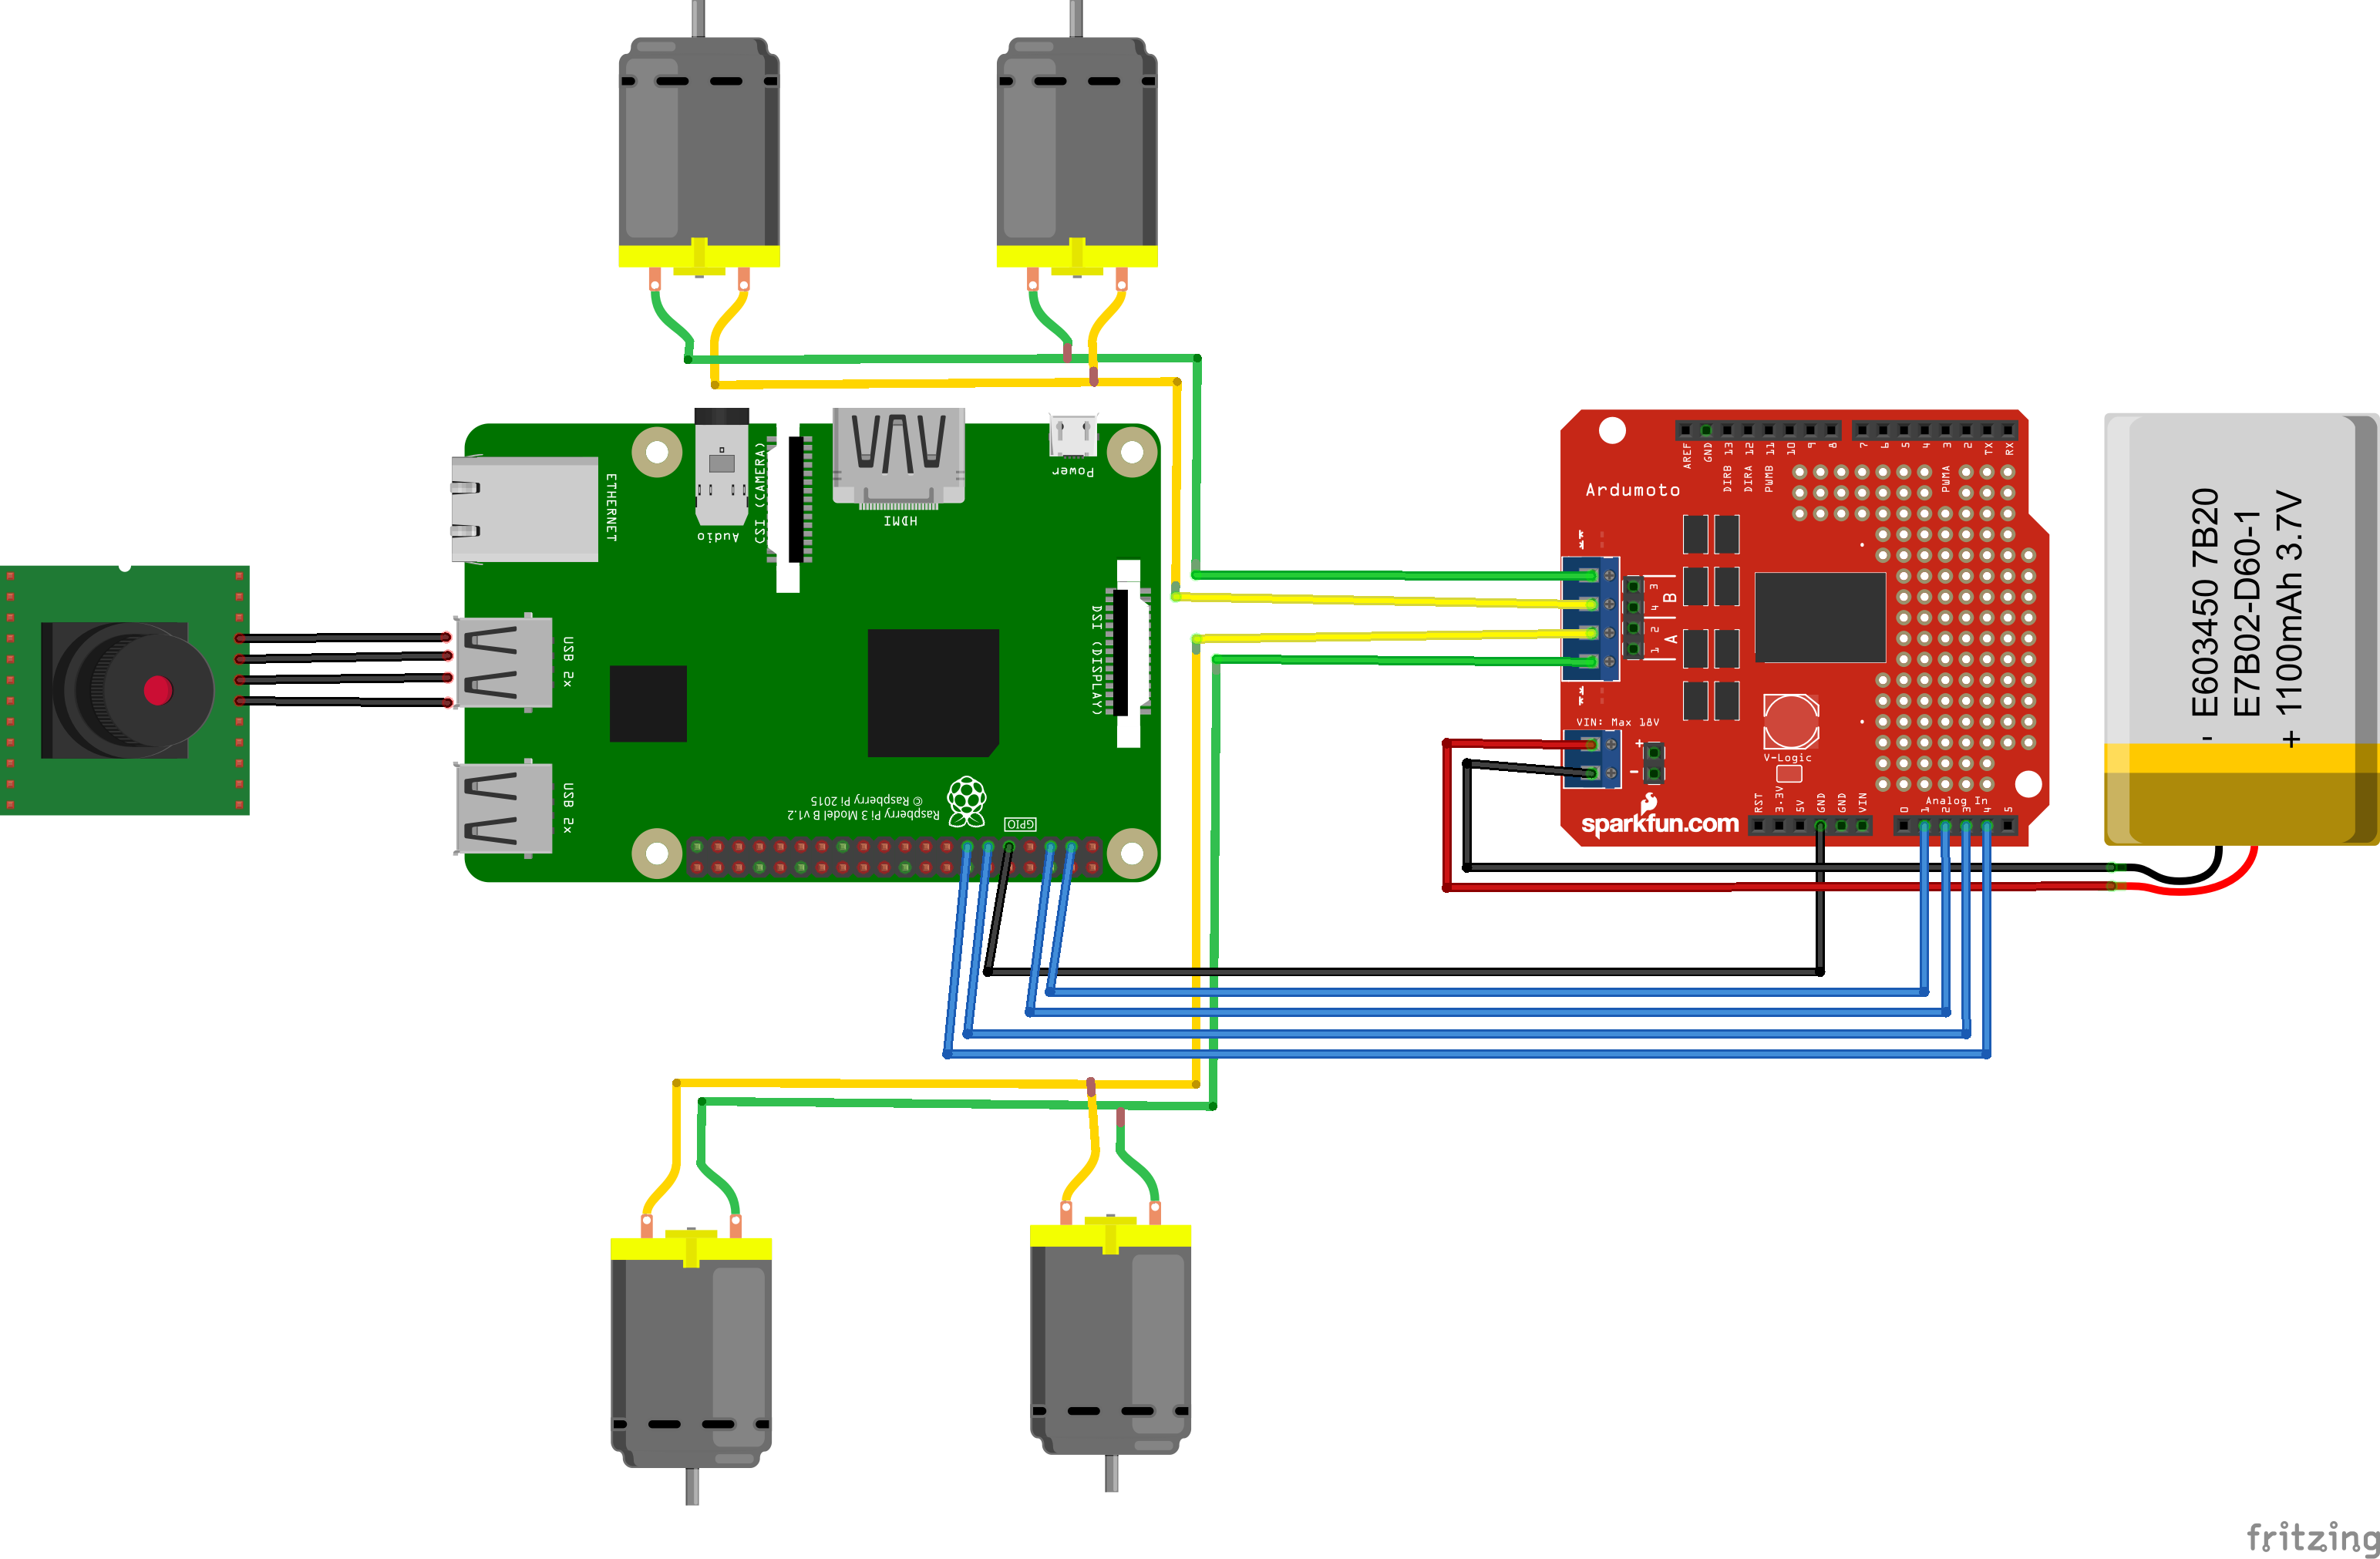
\includegraphics[scale=0.4]{imagenes/robot/robot-esquema.png}
  \end{center}
  \caption{Esquema de conexiones del robot de pruebas.}
  \label{gantt:tareas01}
\end{figure}


    
\section{Software de control}
  

Para la programación del robot se ha empleado el lenguaje de programación JavaScript en un entorno de ejecución Node.js. A continuación se describirá aquellos aspectos más importantes referentes al código
desarrollado para el control del robot.\\

Primeramente se ha realizado la carga de librerías necesarias, entre ellas encontramos:

\begin{itemize}
 \item \emph{pigpio}: Módulo para la comunicación y control de los pines GPIO.
 \item \emph{child process}: El módulo child\_process proporciona la capacidad de generar procesos secundarios. Se ha empleado para la captura de vídeo mediante el lanzado de comandos ffmpeg.
 \item \emph{socket.io}: Biblioteca que establece enlaces bidireccionales en tiempo real y en comunicación basada por eventos.
\end{itemize}


\subsubsection{Entrada/Salida}

En segundo lugar se han definido los diferentes pines GPIO a utilizar y si serán empleados como pines de entrada o de salida:

\begin{lstlisting}[language=JavaScript]
//Pines de la Raspberry Pi connectados al vehículo remoto.
var gpio2 = new Gpio(2, {mode: Gpio.OUTPUT}),
  gpio3 = new Gpio(3, {mode: Gpio.OUTPUT}),
  gpio17 = new Gpio(17, {mode: Gpio.OUTPUT}),
  gpio27 = new Gpio(27, {mode: Gpio.OUTPUT});
\end{lstlisting}


\begin{table}[H]
  \begin{center}
    \begin{tabular}{|p{2.5cm}|p{2.5cm}|p{4.5cm}|}
      \hline
      {\textbf{GPIO}} & \textbf{ Modo } & \textbf{ Control }\\
      \hline
      {\textbf{ 2 }} & { OUTPUT } & { Motores lado derecho }  \\
     \hline
      {\textbf{ 3 }} & { OUTPUT } & { Motores lado izquierdo } \\
      \hline
      {\textbf{ 17 }} & { OUTPUT } & {  Motores lado derecho } \\
      \hline
      {\textbf{ 27 }} & { OUTPUT } & { Motores lado izquierdo } \\
     \hline   
    \end{tabular}
  \end{center}
\caption{ Configuración establecida para los puertos GPIO. }
\end{table}


Si para el vehículo que deseemos programar resultan necesarios más pines tan solo debemos inicializarlos e indicar si van a ser pines de entrada o de salida. Si existen dudas al respecto se puede 
acceder a la documentación de la biblioteca \emph{pigpio} en el siguiente enlace: \url{https://www.npmjs.com/package/pigpio}



\subsubsection{Sockets}


Para la creación del socket basta con la siguiente instrucción, la cual recibe un puerto que utilizará para mantenerse a la escucha: 

\begin{lstlisting}[language=JavaScript]
  var io = require('./node_modules/socket.io').listen(8085, { log: false });
\end{lstlisting}


Con la finalidad de ir capturando los diferentes eventos, se han definido las siguientes funciones para la conexión y desconexión de los clientes:

\begin{lstlisting}[language=JavaScript]

io.sockets.on('connection', function (socket)
{

  //Almacenamiento del número total de clientes conectados.
  sockets[socket.id] = socket;
  console.log("Total clientes conectados : ", Object.keys(sockets).length);
  
  //Envío de un saludo.
  socket.emit('robotmsg', {msg: "!!!HOLA!!!"});


  //Salida de un cliente.
  socket.on('disconnect', function() {
    console.log('Bye!');
    stopStreaming(socket);
  });  
  
}
\end{lstlisting}

Cuando un evento \emph{action} es recibido se activada la función que procesa el comando recibido y activa las salidas correspondientes, la cual establece los pines necesarios a los valores
1 o 0 según el parámetro establecido. A continuación se muestra el ejemplo desarrollado para la activación de los motores en sentido de giro y dirección:\\

\begin{lstlisting}[language=JavaScript]
  // Escucha de comandos.
  socket.on('action', function (data, req, res){

    switch(data) {
      case 'UP':
        gpio2.digitalWrite(1);
        gpio3.digitalWrite(0);
        gpio17.digitalWrite(1);
        gpio27.digitalWrite(0);
        console.log('UP');
        break;
      case 'DOWN':
        gpio2.digitalWrite(0);
        gpio3.digitalWrite(1);
        gpio17.digitalWrite(0);
        gpio27.digitalWrite(1);
        console.log('DOWN')
        break;
      case 'STOP':
        gpio2.digitalWrite(0);
        gpio3.digitalWrite(0);
        gpio17.digitalWrite(0);
        gpio27.digitalWrite(0);
        console.log('STOP');
        break;
      default:
        console.log('command not found');
    }

  });
\end{lstlisting}



\subsubsection{ Streaming de vídeo }



Para el streaming de vídeo desde el robot hacia el cliente conectado se ha empleado las librerías FFmpeg, haciendo uso de su herramienta de línea de comandos.


function startStreaming(socket) {
  //ffmpeg -f video4linux2 -i /dev/video0 -s 300x150 -f mjpeg pipe:1 -b:v 28k -bufsize 28k

  if (running_camera == false){
    console.log('Starting streaming....');
    var args = ["-f", "video4linux2", "-i", "/dev/video0", "-s", "300x150","-f","mjpeg", "pipe:1", "-b:v 28k", "-bufsize 28k"]
    ffmpeg_command = require('child_process').spawn("ffmpeg", args);
    running_camera = true
  }

  ffmpeg_command.on('error', function(err, stdout, stderr) {
    console.log("ffmpeg stdout:\n" + stdout);
    console.log("ffmpeg stderr:\n" + stderr);
    running_camera = false
  });


  ffmpeg_command.on('close', function (code) {
    console.log('ffmpeg exited' + code );
    running_camera = false
  });


  ffmpeg_command.stderr.on('data', function (data) {
    //console.log('stderr: ' + data);
  });

  ffmpeg_command.on('end', function() {
    console.log('Finished');
    running_camera = false
  });

  ffmpeg_command.stdout.on('data', function (data) {
    //console.log('stdout: ' + data);
    var frame = new Buffer(data).toString('base64');
    socket.emit('canvas',frame);
  });

}





\subsubsection{Código de ejemplo completo}

\begin{lstlisting}[language=JavaScript]
 // Start a socket.io server that listens on port 8085.
var io = require('./node_modules/socket.io').listen(8085, { log: false });

// Load required modules.
var sys = require('util'), exec = require('child_process').exec,
    path = require('path'), ffmpeg_command, running_camera = false,
    Gpio = require('pigpio').Gpio;

var sockets = {};

// Pin numbers on the Raspberry Pi connected to the car's remote.
var gpio2 = new Gpio(2, {mode: Gpio.OUTPUT}),
  gpio3 = new Gpio(3, {mode: Gpio.OUTPUT}),
  gpio17 = new Gpio(17, {mode: Gpio.OUTPUT}),
  gpio27 = new Gpio(27, {mode: Gpio.OUTPUT});


console.log('Waiting connection...');

io.sockets.on('connection', function (socket)
{

  sockets[socket.id] = socket;
  console.log("Total clients connected : ", Object.keys(sockets).length);
  socket.emit('robotmsg', {msg: "HELLO!!!"});


  socket.on('disconnect', function() {
    console.log('Bye!');
    stopStreaming(socket);
  });


  socket.on('start-stream', function() {
    startStreaming(socket);
  });


// Listen for direction messages from the app.
  socket.on('action', function (data, req, res){

    switch(data) {
      case 'UP':
        gpio2.digitalWrite(1);
        gpio3.digitalWrite(0);
        gpio17.digitalWrite(1);
        gpio27.digitalWrite(0);
        console.log('UP');
        break;
      case 'DOWN':
        gpio2.digitalWrite(0);
        gpio3.digitalWrite(1);
        gpio17.digitalWrite(0);
        gpio27.digitalWrite(1);
        console.log('DOWN')
        break;
      case 'STOP':
        gpio2.digitalWrite(0);
        gpio3.digitalWrite(0);
        gpio17.digitalWrite(0);
        gpio27.digitalWrite(0);
        console.log('STOP');
        break;
      default:
        console.log('command not found');
    }

  });
});




function stopStreaming(socket) {
  delete sockets[socket.id];
  // no more sockets, kill the stream
  if (Object.keys(sockets).length == 0) {
    if (ffmpeg_command){
      ffmpeg_command.kill();
      running_camera = false;
      console.log('Stop streaming');
    }
  }
}

function startStreaming(socket) {
  //ffmpeg -f video4linux2 -i /dev/video0 -s 300x150 -f mjpeg pipe:1 -b:v 28k -bufsize 28k

  if (running_camera == false){
    console.log('Starting streaming....');
    var args = ["-f", "video4linux2", "-i", "/dev/video0", "-s", "300x150","-f","mjpeg", "pipe:1", "-b:v 28k", "-bufsize 28k"]
    ffmpeg_command = require('child_process').spawn("ffmpeg", args);
    running_camera = true
  }

  ffmpeg_command.on('error', function(err, stdout, stderr) {
    console.log("ffmpeg stdout:\n" + stdout);
    console.log("ffmpeg stderr:\n" + stderr);
    running_camera = false
  });


  ffmpeg_command.on('close', function (code) {
    console.log('ffmpeg exited' + code );
    running_camera = false
  });


  ffmpeg_command.stderr.on('data', function (data) {
    //console.log('stderr: ' + data);
  });

  ffmpeg_command.on('end', function() {
    console.log('Finished');
    running_camera = false
  });

  ffmpeg_command.stdout.on('data', function (data) {
    //console.log('stdout: ' + data);
    var frame = new Buffer(data).toString('base64');
    socket.emit('canvas',frame);
  });

}

\end{lstlisting}

